\documentclass[a4paper]{article}

\renewcommand{\textfraction}{0.15}
\renewcommand{\topfraction}{0.85}
\renewcommand{\bottomfraction}{0.65}
\renewcommand{\floatpagefraction}{0.70}

\usepackage{graphicx}
\usepackage{url}
\usepackage{subfigure}

\usepackage{color}
\definecolor{rltbrightred}{rgb}{1,0,0}
\definecolor{rltred}{rgb}{0.75,0,0}
\definecolor{rltdarkred}{rgb}{0.5,0,0}
%
\definecolor{rltbrightgreen}{rgb}{0,0.75,0}
\definecolor{rltgreen}{rgb}{0,0.5,0}
\definecolor{rltdarkgreen}{rgb}{0,0,0.25}
%
\definecolor{rltbrightblue}{rgb}{0,0,1}
\definecolor{rltblue}{rgb}{0,0,0.75}
\definecolor{rltdarkblue}{rgb}{0,0,0.5}
%
\definecolor{webred}{rgb}{0.5,.25,0}
\definecolor{webblue}{rgb}{0,0,0.75}
\definecolor{webgreen}{rgb}{0,0.5,0}

\usepackage[pdftex,
        colorlinks=true,
        urlcolor=rltblue,               % \href{...}{...}
        anchorcolor=rltbrightblue,
        filecolor=rltgreen,             % \href*{...}
        linkcolor=rltred,               % \ref{...} and \pageref{...}
        menucolor=webblue,
        citecolor=webgreen,
        pdftitle={MTF Mapper documentation},
        pdfauthor={F. van den Bergh},
        pdfsubject={MTF Mapper documentation},
        pdfkeywords={MTF MTF50 acuity sharpness slanted edge autfocus},
        pdfpagemode=UseNone,
        bookmarksopen=true]{hyperref}


\addtolength{\textwidth}{2cm}
\addtolength{\hoffset}{-1cm}
\setlength{\parindent}{0pt}
\setlength{\parskip}{1ex}

\title{MTF Mapper user documentation}
\author{F. van den Bergh (fvdbergh@gmail.com)}

\begin{document}
\maketitle

\tableofcontents

\section{Overview}
The MTF mapper package offers a collection of tools to measure Modulation
Transfer Function (MTF) values across edges in images. It does this by computing the edge
spread function of a step edge in an image, using the method described by
Khom \cite{khom} (Section~\ref{sec:description} provides a brief overview).

MTF mapper offers fully automated operation, producing the following
outputs:
\begin{enumerate}
    \item Annotated images, where the MTF50 value of an edge is printed on top
of the edge itself;
    \item Profile data sets, where the MTF50 values are represented in a
one-dimensional projection of the image. This is the tool you want if you
are interested in objectively adjusting your DSLR autofocus fine-tuning (see
Section~\ref{sec:autofocus} for details of the method).
    \item MTF surface images, where you can visualise the MTF50 values
across the focal plane, to see the image centre MTF50 relative to edge MTF50,
for example.
\end{enumerate}

MTF mapper expects images containing dark rectangular objects on light
backgrounds; the objects can be slightly out-of-square, e.g., trapezoids or
parallelograms, provided the interior angles are at least reasonably close
to 90$^\circ$.

Special test charts are required for Profile mode.
Section~\ref{sec:profile_mode} describes them in more detail.

Special test charts are also required for MTF surface mode.
Section~\ref{sec:surface_mode} describes them in more detail.

\section{Modes}
The main tool in the package is called \texttt{mtf\_mapper}; you could simply
invoke it as 
\begin{verbatim} mtf_mapper <image>
\end{verbatim}
where \texttt{<image>} can be in a variety of image formats, including 
PNG, JPG, TIFF, PNM, and more. After successfull extraction of MTF50 values
from the edges found in the image, the information is made available in
several forms, called ``modes'', detailed next.

\subsection{Annotation mode (\texttt{-a} or \texttt{--annotate} flag)}
\label{sec:annotation_mode}
No explanation required, really. Input images are searched for rectangular
objects. Once found, the MTF50 value will be computed across each edge of
all the rectangular objects. The resulting value is drawn on top of each
edge, and the result saved as \textrm{annotated.png} by default.

\subsection{Profile mode (\texttt{-p} or \texttt{--profile} flag)}
\label{sec:profile_mode}
Using a special test chart illustrated in Figure~\ref{fig:profile_test_chart}, 
the program will construct a profile such as the one shown in 
Figure~\ref{fig:sample_profile}, which was derived from the original image
shown downsampled in Figure~\ref{fig:profile_test_chart}(b). The chart should
be photographed at a $45^\circ$ angle.

\begin{figure}
\centering
\subfigure[Perspective chart]{
  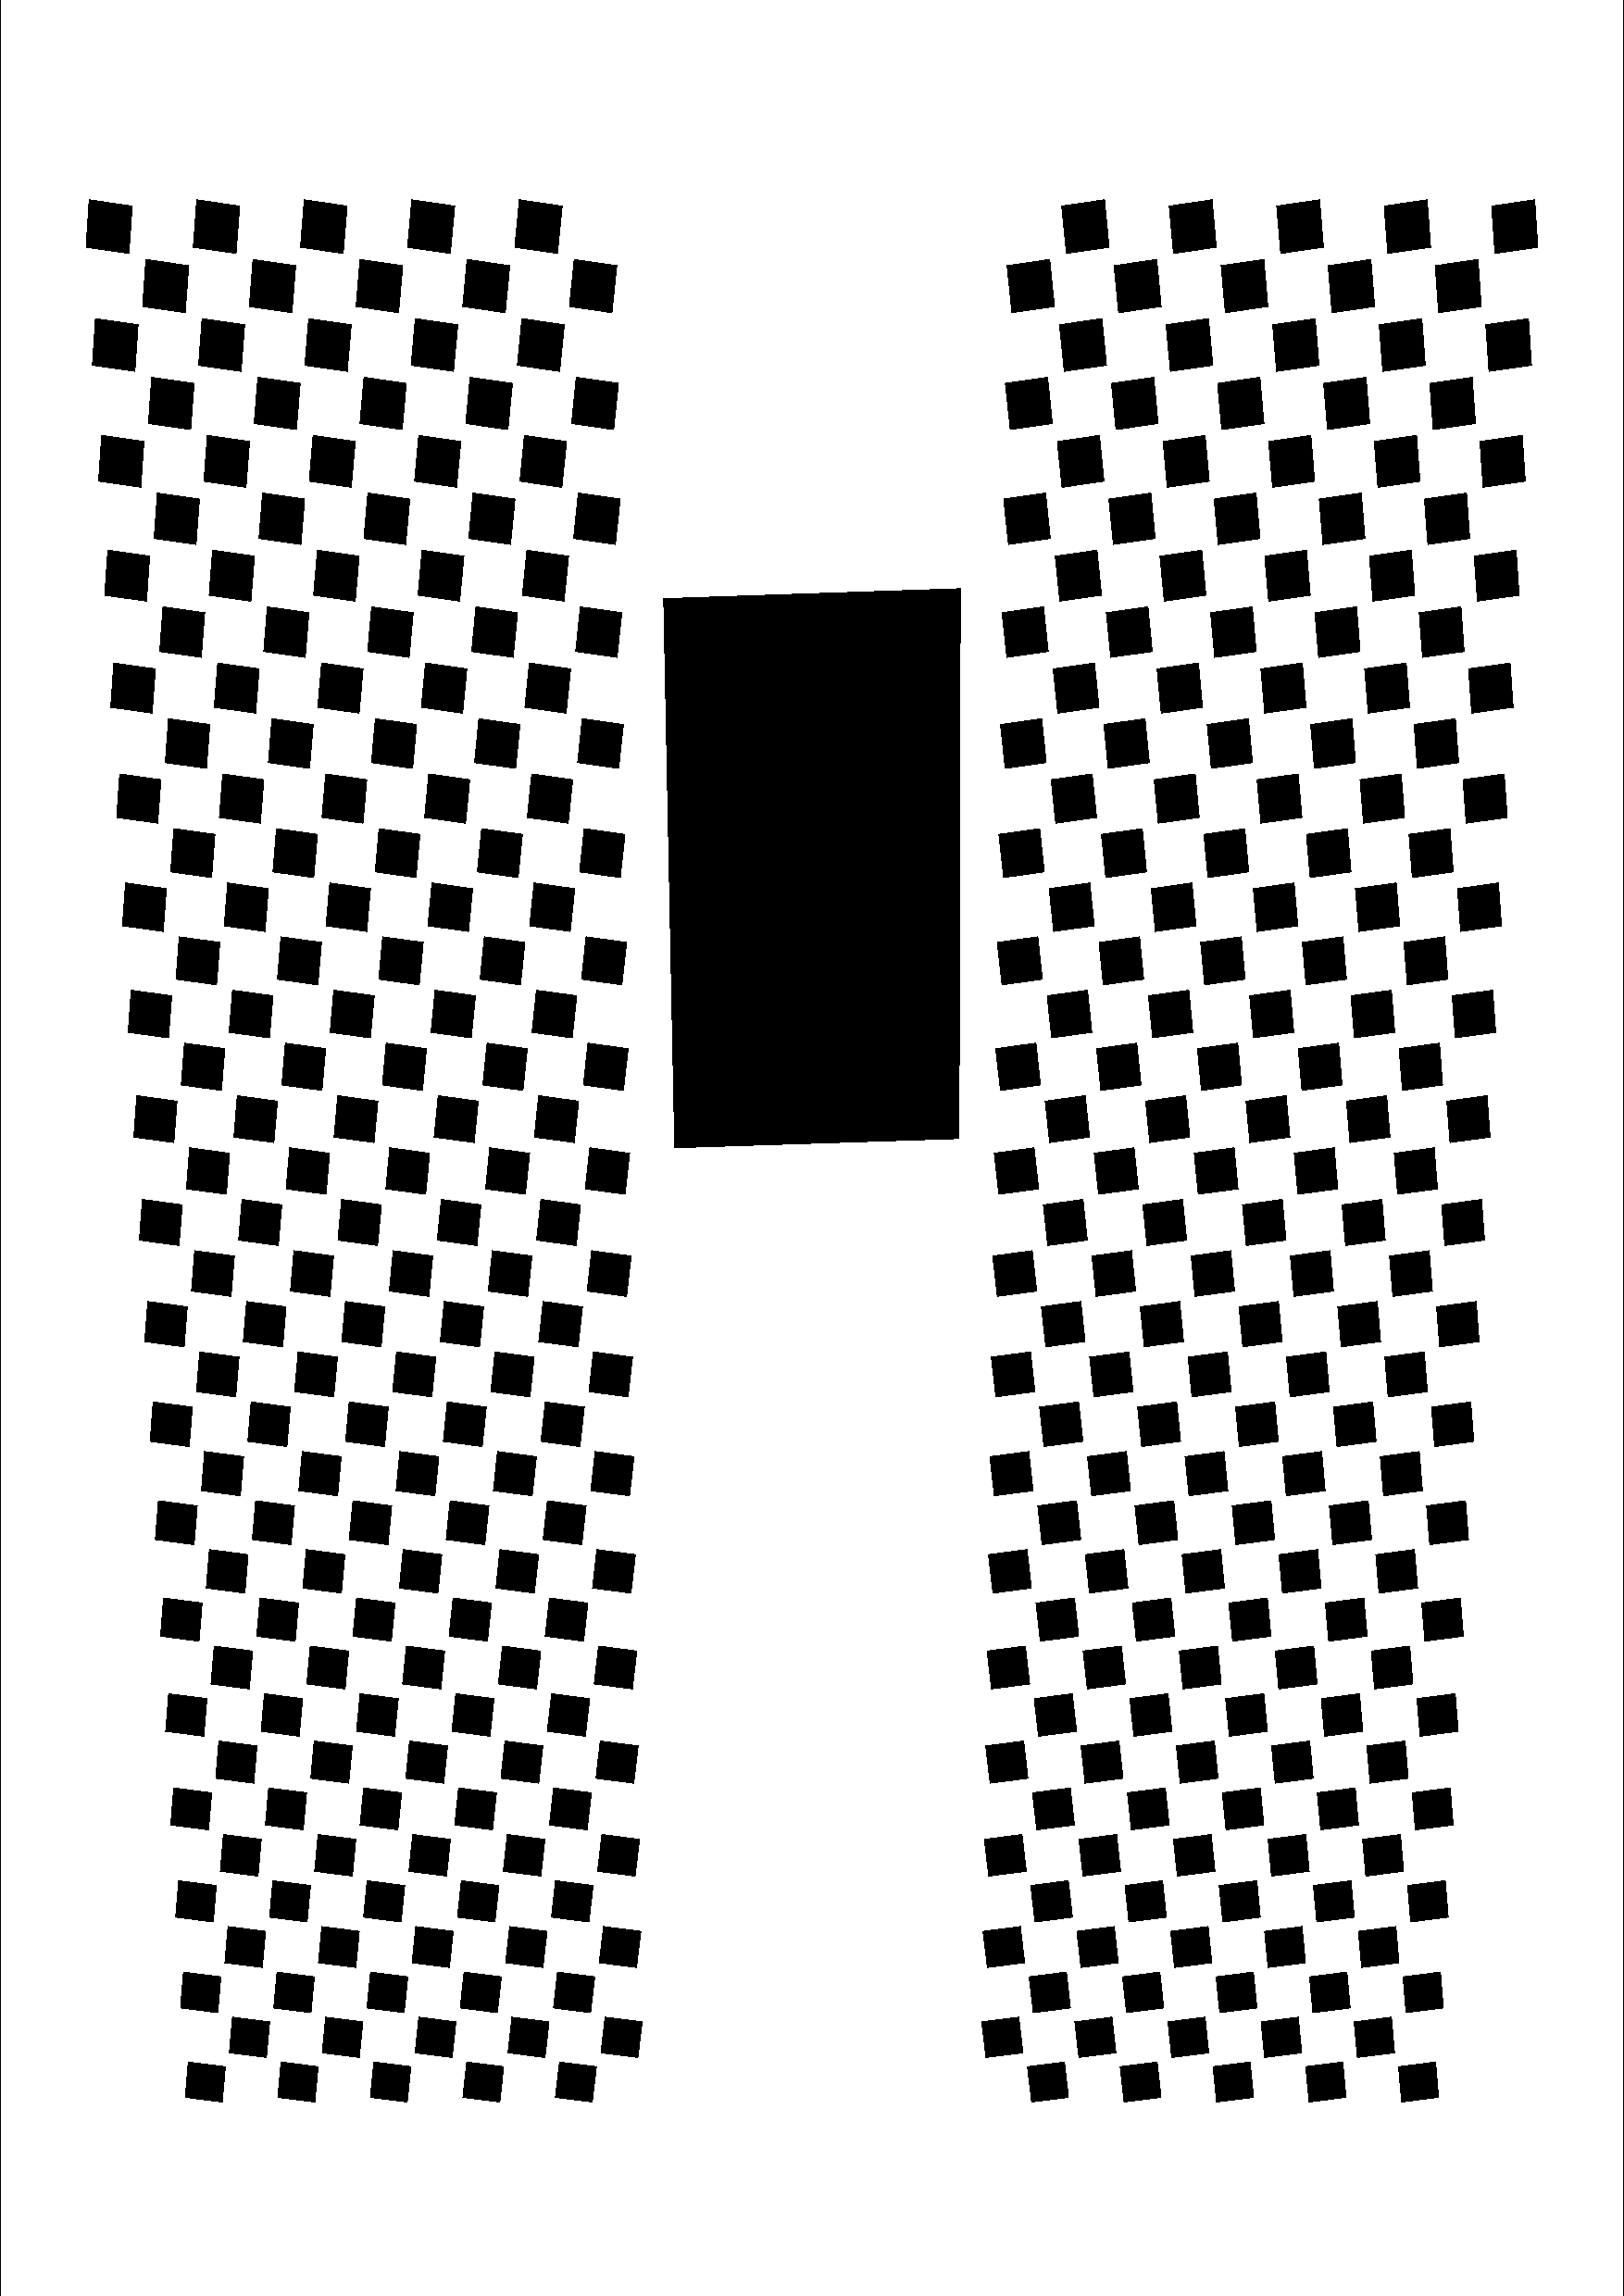
\includegraphics[width=0.3\textwidth]{figures/mtf_profile_test_chart}
}
\subfigure[A photo of this type of chart at $45^\circ$]{
  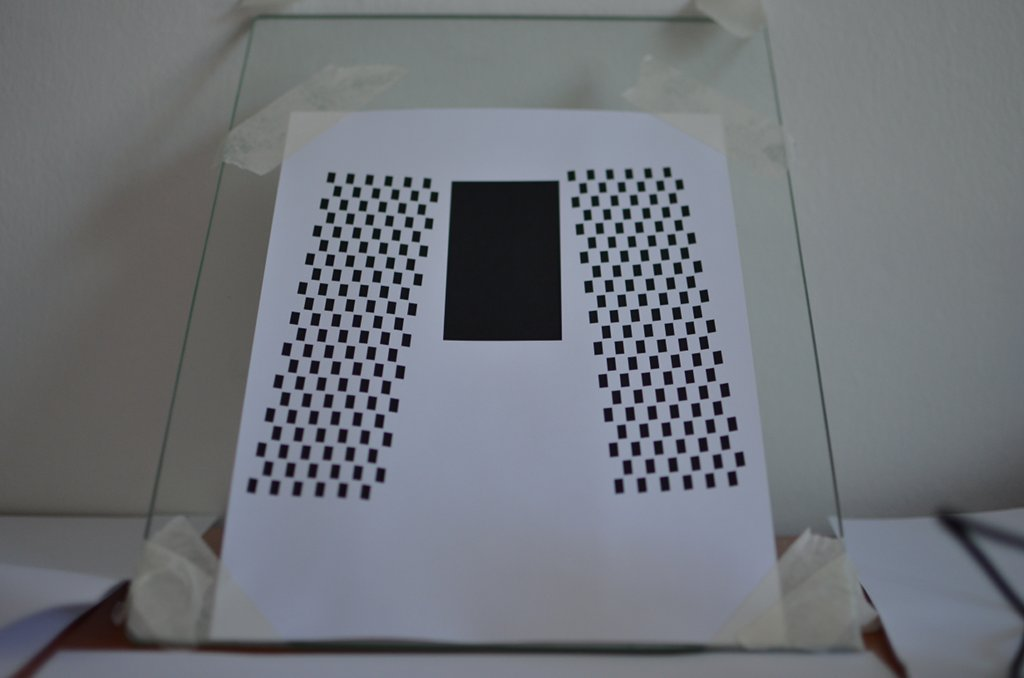
\includegraphics[width=0.65\textwidth]{figures/perspective_sample_photo}
}
\caption{An illustration of the type of test chart used in \emph{profile}
mode.}
\label{fig:profile_test_chart}
\end{figure}

\begin{figure}
\centering
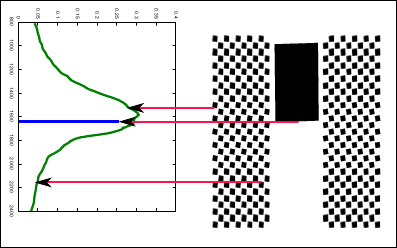
\includegraphics[width=0.8\textwidth]{figures/profile_construction}
\caption{How the profile is constructed: MTF50 values are collapsed
horizontally onto the $y$-axis to form the profile.}
\label{fig:profile_construction}
\end{figure}

\begin{figure}
\centering
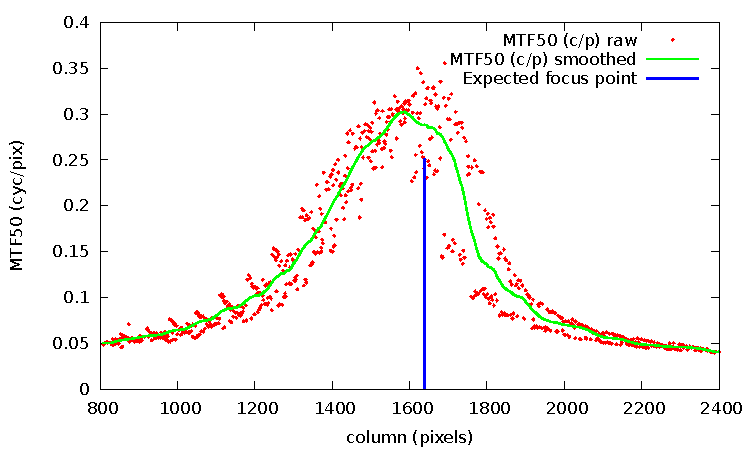
\includegraphics[width=0.95\textwidth]{figures/sample_profile}
\caption{Example of profile generated by MTF mapper. Derived from the image
shown in Figure~\ref{fig:profile_test_chart}(b).}
\label{fig:sample_profile}
\end{figure}

The large central block in the chart (Figure~\ref{fig:profile_test_chart}) 
is called the reference block, and the edge of this block closest to the
centre of the chart (the bottom edge in Figure~\ref{fig:profile_test_chart})
is called the \emph{reference edge}.
The MTF50 values computed across the edges of all the blocks in the image
are projected onto the $y$-axis of the image, thus forming a new set of data
points of the form ($y$-value, MTF50 value). This process is illustrated in
Figure~\ref{fig:profile_construction}. The idea is that about half of the
chart will be in front of the plane of focus, and the other half behind. If
the depth of field is sufficiently shallow, then the closest and furthest of
the small blocks will be noticibly blurry. By projecting the measured
sharpness value (MTF50) of each block along horizontal lines
(Figure~\ref{fig:profile_construction}), we obtain a roughly bell-shaped
profile as shown in green on the left. The peak of this curve corresponds to the plane
of focus, and blocks that are further or closer than this plane are out of
focus to some degree. The blue line indicates the position of the
\emph{reference edge}.

A complete profile in its usual orientation is shown in 
Figure~\ref{fig:sample_profile}. The red dots represent individual MTF50
measurements, and the green curve is merely a smoothed representation of the
same data.

Generally, \emph{Profile} mode is only intended to be used to calibrate or
evaluate the autofocus sensor of a DSLR; the details of this process are
described in Section~\ref{sec:autofocus}. The objective is to adjust the
camera so that the blue line (reference edge, or focus position) lines up
with the peak of the green curve / red point cloud. If the blue line is far
from the peak, then you are experiencing either front- or back-focus. If
your chart was positioned at a $45^\circ$ angle so that the bottom edge 
was closer to you, then front focus would mean that the blue line appears to
the left of the peak in the green curve. This depends on the orientation of
the camera, though, so you may want to take a look at the annotated image
(see Section~\ref{sec:annotation_mode}) to orient yourself. The trick is to
remember that the peak in the green curve (or red point cloud) corresponds
to the \emph{actual} plane of focus, whereas the blue line corresponds to
where MTF Mapper \emph{thinks} you have placed the autofocus sensor when you
framed the shot.

\subsection{MTF Surface mode (\texttt{-s} or \texttt{--surface} flag)}
\label{sec:surface_mode}
%
\begin{figure}
\centering
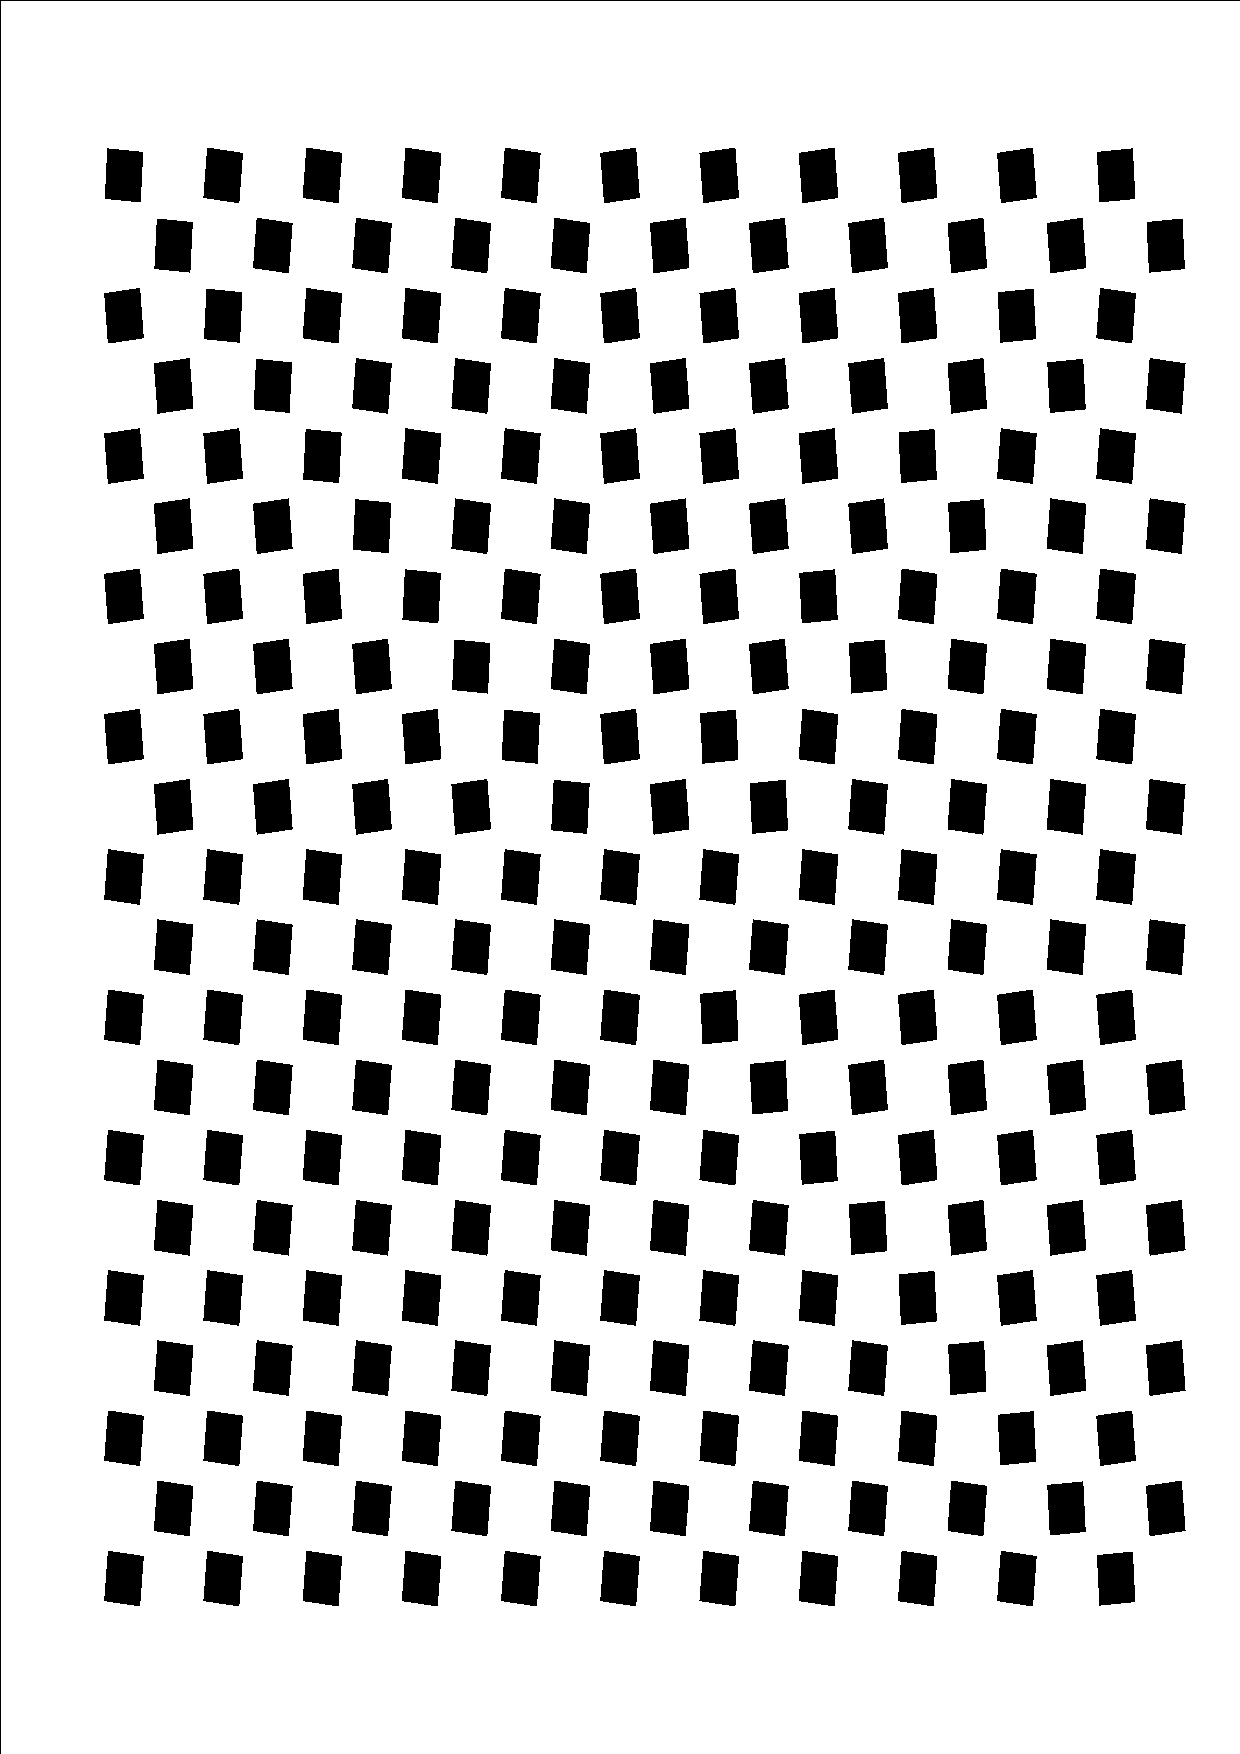
\includegraphics[width=0.5\textwidth,angle=90]{figures/mtf_surface_test_chart.pdf}
\caption{Example of an MTF surface mode test chart}
\label{fig:surface_test_chart}
\end{figure}
%
Using any test chart with a regular grid of rectangles (as illustrated in
Figure~\ref{fig:surface_test_chart}), you can measure the acuity of your
lens/camera system as it varies across the focal plane. Just shoot the chart
at a reasonable distance, making sure that it covers the entire viewfinder.
For optimal accuracy, the orientation of the blocks in the chart should be
approximately $5^\circ$--$15^\circ$ with respect to the pixel rows or columns.
The charts produced by the \texttt{generate\_test\_chart} program included
with MTF Mapper already take care of this, so you should try to capture the
chart as straight as possible. Do note that this becomes more critical at
higher sharpness settings, i.e., if you have a really sharp lens and you are
sharpening your images excessively, then you have to observe the orientation
of the chart carefully. For typical lenses and unsharpened images, 
chart alignment is not critical.

\begin{figure}
\centering
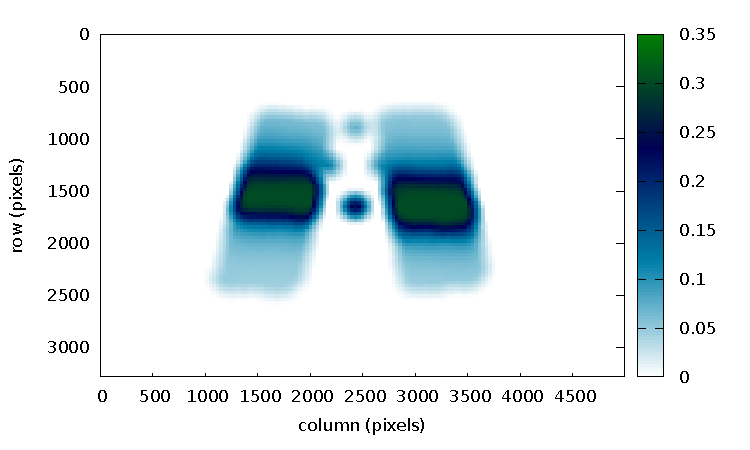
\includegraphics[width=0.95\textwidth]{figures/sample_grid_image}
\caption{Example of MTF50 image generated by MTF mapper}
\label{fig:sample_grid_image}
\end{figure}

\begin{figure}
\centering
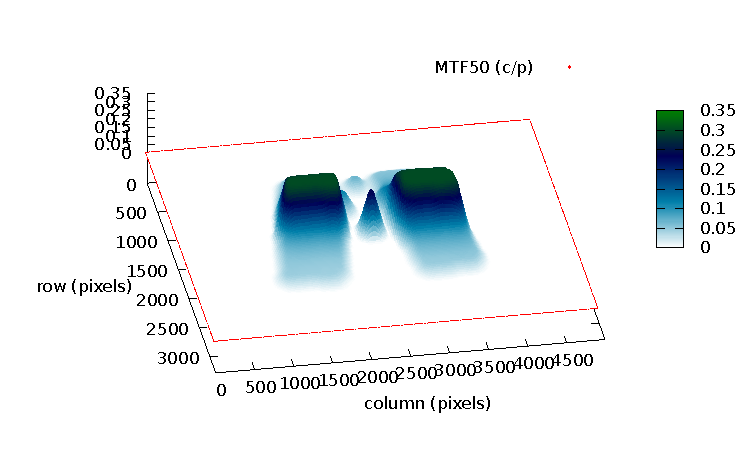
\includegraphics[width=0.95\textwidth]{figures/sample_grid_surface}
\caption{Example of MTF50 surface generated by MTF mapper}
\label{fig:sample_grid_surface}
\end{figure}

Surface mode produces two images: one representing a 2D
representation of MTF50 values across your image, and another showing the
same data rendered as a 3D surface. Examples of both can be seen in
Figures~\ref{fig:sample_grid_image} and \ref{fig:sample_grid_surface}. These
images were obtained using a photo of the Profile mode test chart of
Figure~\ref{fig:profile_test_chart}, just because it is a bit more
interesting to look at. Since this chart was photographed at a $45^\circ$
angle, the sharpest focus is observed around the position of the reference
edge (seen as the isolated conical peak in
Figure~\ref{fig:sample_grid_surface}, and corresponding circular dot in the
centre of Figure~\ref{fig:sample_grid_image}). Focus deteriorates as you
move up or down along the image (corresponding to moving further from the
plane of focus), resulting in a decrease in MTF50 values. Incidentally, this
particular lens is now fairly close to optimally calibrated, since the
sharpest focus region is relatively well aligned with the position of the
\emph{reference edge}.


\section{Autofocus fine-tuning}
\label{sec:autofocus}
%
\begin{figure}
\centering
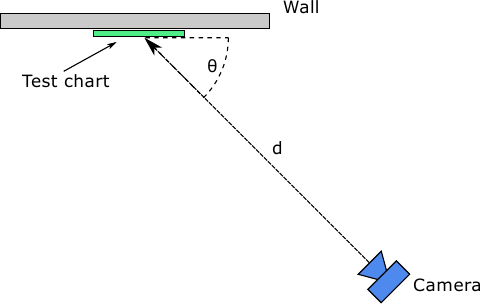
\includegraphics[width=0.65\textwidth]{figures/af_setup}
\caption{Illustration showing the top view of the autfocus calibration
set-up}
\label{fig:af_setup}
\end{figure}
%
\begin{figure}
\centering
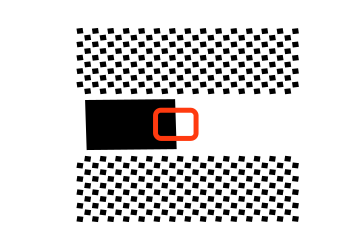
\includegraphics[width=0.65\textwidth]{figures/af_sensor_placement}
\caption{Where to place your autofocus sensor}
\label{fig:af_sensor_placement}
\end{figure}
%
The following steps can be used to calibrate the autofocus fine-tuning of a
DSLR:
\begin{enumerate}
    \item Figure~\ref{fig:af_setup} illustrates the basic set-up. The
distance $d$ is the ``distance to chart'', and the angle $\theta$ is the
``angle with respect to the test chart''.
    \item Print out the test chart at a large enough scale. Ideally, your
test chart must be large enough so that you can use it at a distance of
$30\times$ the focal length of your lens. Position your camera so that you
see the chart from an angle of at least $45^\circ$ --- the idea is that you
want some of the small blocks to be in front of the plane of focus, and some
of the blocks behind the plane of focus; this is easier to achieve at angles
of $45^\circ$ and smaller. The reference edge (Section~\ref{sec:profile_mode}) should be
exactly at the plane of focus, but since you are reading this, I take it you
are still trying to adjust the autofocus fine-tuning to achieve this.
    \item Using a tripod (and remote release / timed release), take a
picture of the test chart \emph{with your chosen (centre recommended)
autofocus sensor straddling the edge of the reference block}, as illustrated
in Figure~\ref{fig:af_sensor_placement}. Take care that the autofocus sensor
is sufficiently far away from other edges (e.g., the horizontal edges of the
reference block in Figure~\ref{fig:af_sensor_placement}, or any of the small
blocks). Keep in mind that the actual sensing area of the autofocus sensor
is typically larger than the reticule you see in the viewfinder, so leave
some padding.
    \item Feed the captured image through MTF mapper to produce a profile
(such as illustrated in Figure~\ref{fig:sample_profile}. The vertical red
line denotes the position of the autofocus reference edge (at least, the one
you should have been using to focus \ldots). The green curve (or blue
points) records the MTF50 values measured along the $y$-axis of the image.
Since the test chart was at a $45^\circ$ angle with respect to the lens
axis, the $y$-axis of the image is a measure of the distance from the
camera. MTF50 values measured at different $y$-values thus indicate the
sharpness, or degree of focus, at that specific distance from the camera.
The peak of the green curve represents the plane of focus --- the objective
is to line up the peak of the green curve with the red vertical line.
    \item This procedure should now be repeated at various autofocus
fine-tuning settings on your camera. You should be able to see the peak of
the green curve shift left or right as you adjust this value. I recommend
capturing your images in batches, first stepping your autofocus fine-tuning
through the range in large steps, running the images through MTF mapper, and
then repeating this in the optimal range with smaller steps until you are
satisfied that you have calibrated your autofocus fine-tuning to the desired
level of accuracy.
\end{enumerate}

\subsection{Caveats and disclaimers}
Please note that this procedure of calibrating autofocus fine-tuning on your
DSLR is based on some of my own assumptions, which have not been tested
rigorously before the release of this software. Here follows some
background; you are most welcome to skip this section.

Phase-detection autofocus in DSLR cameras works by collecting light from
opposite sides of the lens (the aperture, really), if the article on
wikipedia is
accurate\footnote{\url{http://en.wikipedia.org/wiki/Autofocus}}. These two
beams of light are steered to two independent linear sensors --- I suspect
that they are simply small strip-like CMOS sensors nowadays. Using
cross-correlation, the AF module then measures the phase shift between the
data collected from the two linear sensors; this phase shift will directly
correspond to the degree of defocus. With this information, the AF module
can then drive the AF motor by approximately the correct amount to
elliminate the phase difference between the signal received by the two
linear sensors, which should bring the object under the relevant AF sensor
into focus.

So the real question is: what algorithms do the AF modules really use to
measure the phase shift? Well, I currently do not know. If you design AF
modules, please fill me in, and I can update my test charts to agree more
closely with what the AF modules expect to see. Many AF test charts on are
available on the internet, however, most of them use thick line (bar-shaped)
target to draw the AF sensor's attention. Someone on the internet (now,
there is a reference you can count on) pointed out that bar targets are a
poor choice, because they may be too thin for the AF sensor to detect. I
found this argument appealing, because the AF sensor must have limited
resolution. There is an additional problem with a bar target: which edge of
the bar target is the AF module going to focus on? And this process led me
to the design of my own test charts. Rather than using a bar as an AF
target, why not use a step edge? If the AF module really does use
cross-correlation to measure the phase difference, then a step edge would
produce the best possible results. There would also be not ambiguity as to
where the sensor is focussing, since the step edge only has one feature to
focus on.

Well, it seems to work. Until someone can point me in the right direction, I
am simply assuming that the step edge provides a good target for modern AF
sensors. It certainly seems that my own DSLRs have no problem focussing on
the step edge.

I also found it annoying to have to use visual inspection to determine
whether I have set the autofocus fine-tunining optimally. Visual
inspection certainly is a quick way to evaluate the results in the field, but I want to see some
objectve data. I want to \emph{know} that I have calibrated my lenses
perfectly. Anyhow, if you have made it this far, you probably understand.
MTF50 is certainly not the final word on image acuity (read the excellent
Zeiss papers for a start), but it does provide a reasonable relative measure
for the autofocus calibration problem. The MTF50 estimates extracted by MTF
Mapper are reasonable accurate (see Section~\ref{sec:accuracy}), at least as
far as internal consistency goes with my own edge image generator. You
should be able to obtain repeatable results within a 5\% relative margin.

Lastly, you should know one very important thing about autofocus systems:
they are not perfect. The tollerances of the AF system (AF module, lens
drive accuracy, etc.) are such that they strike a balance between speed and
accuracy. In other words, the AF system only takes one stab at the problem:
one phase difference measurement results in one focus motor action. The
implcation of this is that the AF system will only adjust focus so that it 
is ``good enough''. The AF system will only adjust focus up to the point
where the circle of confusion drops below the specified limit. I do not have
solid references on this, but I gather that the specification is for
acceptably sharp $10\times8$ prints. Working backwards, this translates into
a buffer of focus positions around the optimal focus position. The AF system
may stop anywhere within this buffer zone, having complied with the
specifications. With MTF mapper, you can empirically observe this effect:
manually set focus to infinity, switch to AF, capture image. Now select near
focus (manually), switch to AF, capture image. Comparing the profile plots
of produce by MTF mapper you should be able to see which image was captured
from which direction, and the distance between the peaks in the profiles
should roughly correspond to this ``zone of acceptable focus'' for that
subject distance and magnification.

%TODO: examples

\section{Other MTF mapper utilities}
Two additional utilities are included in the MTF mapper package.
\subsection{Rectangle generator}
\label{sec:rectangle_generator}
The \texttt{generate\_rectangle} utility will create a synthetic image of a
rectangle, sampled with a specified Gaussian point spread function. The
rectangle images generated with this utility therefore have a known MTF50
value, which was calculated analytically.

In the current implementation, the Gaussian noise that is optionally added
to the image is not taken into consideration in the analytical calculation
of the expected MTF50 value. This noise certainly makes it more challenging
for software tools to compute the MTF50 values from the generated images,
but it should not bias the result in any way. 

Either way, the \texttt{generate\_rectangle} utility is useful during
testing, and can be used to cross-calibrate the \texttt{mtf\_mapper} utility
with other packages available for computing MTF50 values. (If you have
access to Imatest, please send me some results. Your feedback will help to
improve MTF Mapper).

\subsection{Test chart generator}
The \texttt{generate\_test\_chart} utility can be used to generate SVG files
containing various test charts. Currently, it can generate ``perspective''
charts that are suitable for DSLR autofocus calibration, as well as
empirical measurements of the depth of field of your equipment. It can also
generate ``grid'' charts that contain squares arranged in a regular grid,
which can be used to measure the flatness of field of your
equipment.

Currently, the MTF mapper utilities do not separate MTF50 values into
sagittal and meridional orientations, although such an option would be
relatively straightforward to add, and is planned for a future version.

\section{Frequently Asked Questions}
A bit of a misnomer, since I have yet to receive actual questions :)
\begin{enumerate}
  \item Your program gave me a value of $x$ cycles per pixel. Is this any
good? \emph{Answer}: According to Norman Koren
(\url{http://www.imatest.com/guides/modules/sfr}), a value of 0.33 cycles
per pixel is pretty good \emph{for unsharpened raw images} (emphasis mine).
This seems to roughly agree with what I see on a Nikon D7000 with the Nikkor
35 mm f/1.8 prime. Keep in mind that a Bayer colour filter sensor camera
will never be able to give you ``perfect'' MTF50 values of 0.5 c/p, and that
anything above 0.25 c/p is actually pretty good (before sharpening), 
all things considered.
  \item Cycles per pixel? I wanted lw/ph or lp/mm! \emph{Answer}: Maybe I
will add support in future versions, but you can convert manually using the
following relationship:
    \begin{eqnarray}
	\mathrm{MTF50}_{\mathrm{lp/mm}} = 
	  \frac{\mathrm{MTF50}_{\mathrm{c/p}} \times h_{\mathrm{pixels}}}{h_{\mathrm{mm}}} \\
        \mathrm{MTF50}_{\mathrm{lw/ph}} = 2 \times \mathrm{MTF50}_{\mathrm{c/p}} \times h_{\mathrm{pixels}} 
    \end{eqnarray}
where $h_{\mathrm{mm}}$ is the image height in mm, and $h_{\mathrm{pixels}}$
is the image height in pixels.
\end{enumerate}

\appendix
\section{Internal workings}
\label{sec:description}
Here is a brief outline of how MTF Mapper works:
\begin{enumerate}
    \item The input image is read in, and converted to grayscale (using
OpenCV's default colour matrix). If the input image is an 8-bit image, the
pixel intensities are scaled up to 16 bits; the default is to assume that
8-bit images are sRGB gamma corrected, so the values are linearised while
begin scaled to 16 bits. If the input image has a pixel bit depth of 16
bits, no gamma conversion or scaling is applied.
    \item The image is thresholded using Bradley's adaptive thresholding 
algorithm \cite{bradley}. This is done to identify all the dark objects in
the image.
    \item The thresholded image is then scanned to extract all the connected
components using the method of Chang \textit{et al.}\cite{chang}. This step
gathers the boundary lists of all the dark objects in the image.
    \item The image gradient is computed on the original input image. This
is combined with the object boundary lists to identify all
roughly-rectangular objects (called blocks in the sequel).
    \item For each edge of each detected block, the MTF50 value is computed
as follows (roughly the method of Khom \cite{khom}):
	\begin{enumerate}
	  \item Define a rectangular buffer region that is aligned with and
centered over each edge. The width of this buffer is 32 pixels.
	  \item Compute a reasonable estimate of the orientation of the edge
(using the image gradient information).
	  \item Extract the intensity values of each pixel within the
rectangular buffer, and project the coordinates of this pixel onto the
direction normal to the edge.
          \item Systematically refine the edge normal to minimise the
difference between sequential projected values; this effectively optimises
the edge normal estimate.
	  \item For each pixel in the buffer, record a pair of values
(\textsf{distance}, \textsf{intensity}), where \textsf{distance} denotes the
length of the pixel coordinates projected onto the edge normal, and
\textsf{intensity} represents the actual pixel intensity value. Note that
the distance values are unevenly sampled. These values are a representation
of the edge spread function (ESF).
	  \item Perform LOESS fitting using a linear model to resample the 
(\textsf{distance}, \textsf{intensity}) values to a regular grid. The
resampled points are generated at a spacing of 1/32 pixels, i.e., the
profile is oversampled at a factor of 32. In addition, the derivative of the
ESF is not computed with discrete differentiation; instead, the slope of the
local linear fit is used to construct the line spread function (LSF) directly.
	  \item Apodization is performed by windowing the resampled LSF with
a Hamming window.
	  \item An FFT is computed on the resampled points, and the
normalised FFT magnitude sequence is calculated.
	  \item The frequency at which the FFT magnitude sequence reaches a
value of 0.5 is computed using linear interpolation, yielding the MTF50
value.
	  \item A 7th-order polynomial is used to correct any remaining
systematic bias. Pathologically poor edge orientations are identified, and
suppressed; these are around $22^\circ$ and $45^\circ$ degrees with respect
to either the vertical or horizontal image directions.
	\end{enumerate}
    \item The computed MTF50 values are then rendered in various ways,
depending on which output options are selected.
\end{enumerate}

\section{Accuracy}
\label{sec:accuracy}
The accuracy of the MTF50 estimates produced by MTF Mapper depends on the
following factors:
\begin{enumerate}
  \item Image resolution, and resulting edge length
  \item Image noise levels
  \item Image edge contrast (combined with noise levels, expressed as
  Signal-to-Noise Ratio, SNR)
  \item Edge orientation relative to horizontal or vertical directions
  \item Edge MTF50 value --- the sharper the edge, the more critical the
  above factors become
\end{enumerate}

\begin{figure}
\centering
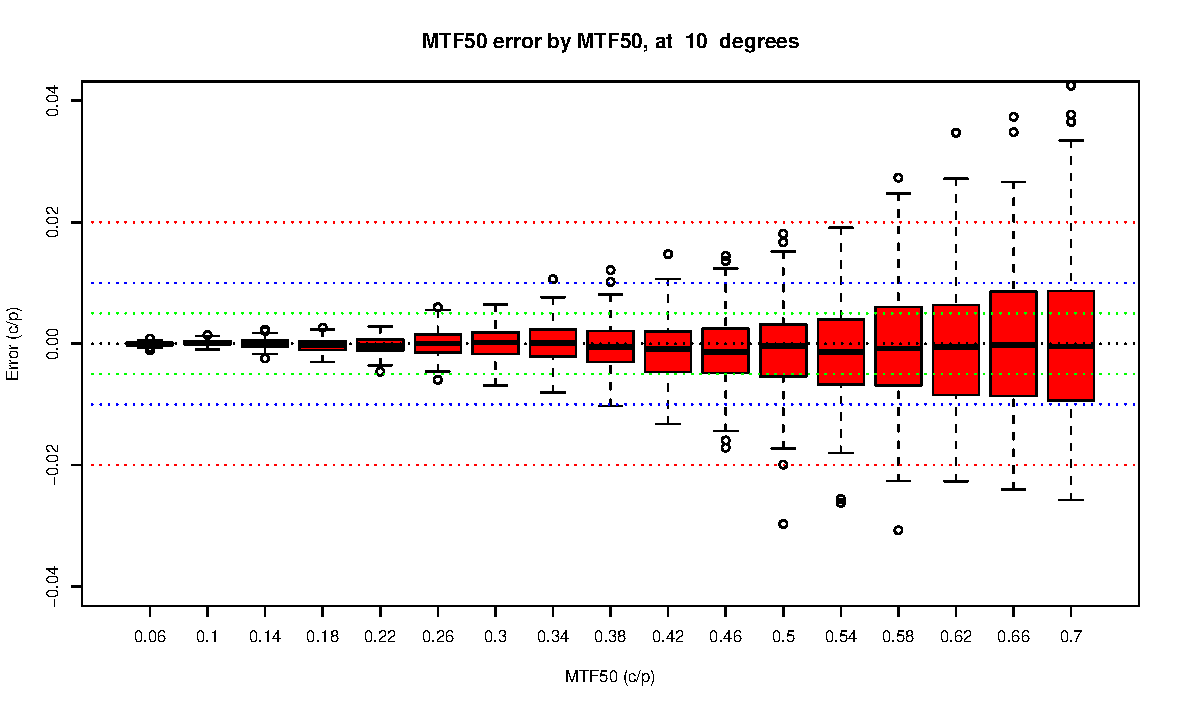
\includegraphics[width=0.95\textwidth]{figures/accuracy_plot_a10_90}
\caption{Error in MTF50 estimate for $10^\circ$ edges, SNR=90}
\label{fig:mtf_accuracy_a10_snr90}
\end{figure}

\begin{figure}
\centering
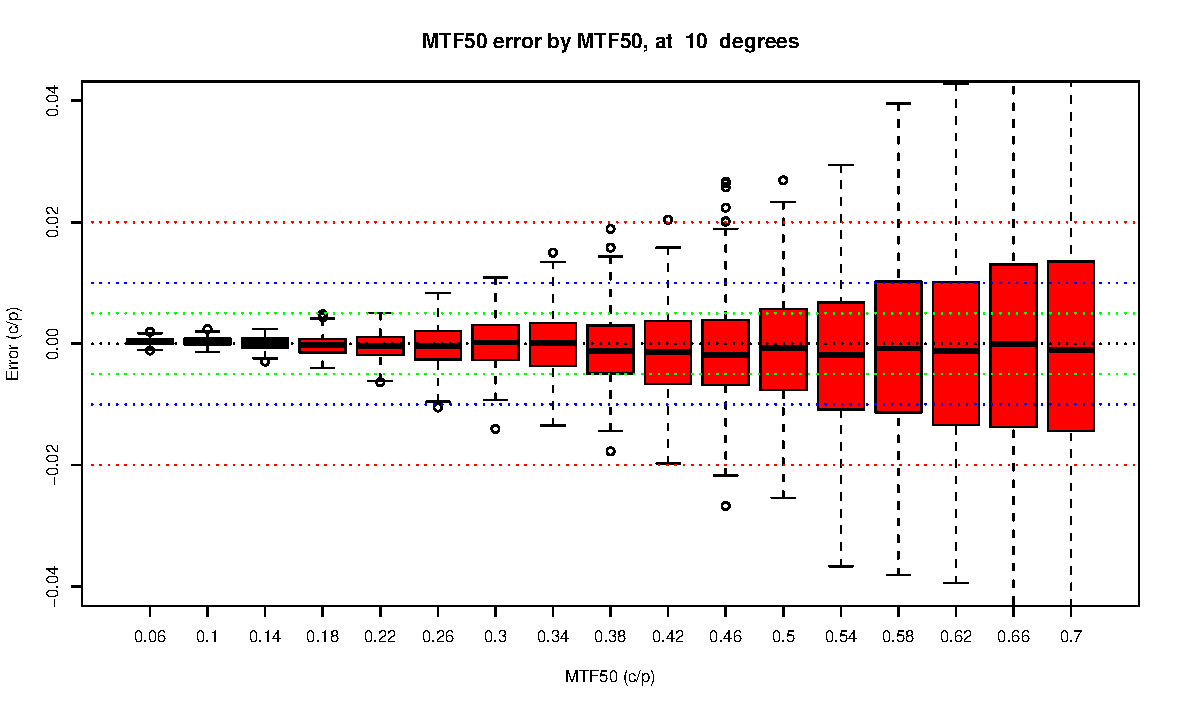
\includegraphics[width=0.95\textwidth]{figures/accuracy_plot_a10_57}
\caption{Error in MTF50 estimate for $10^\circ$ edges, SNR=57}
\label{fig:mtf_accuracy_a10_snr57}
\end{figure}

\begin{figure}
\centering
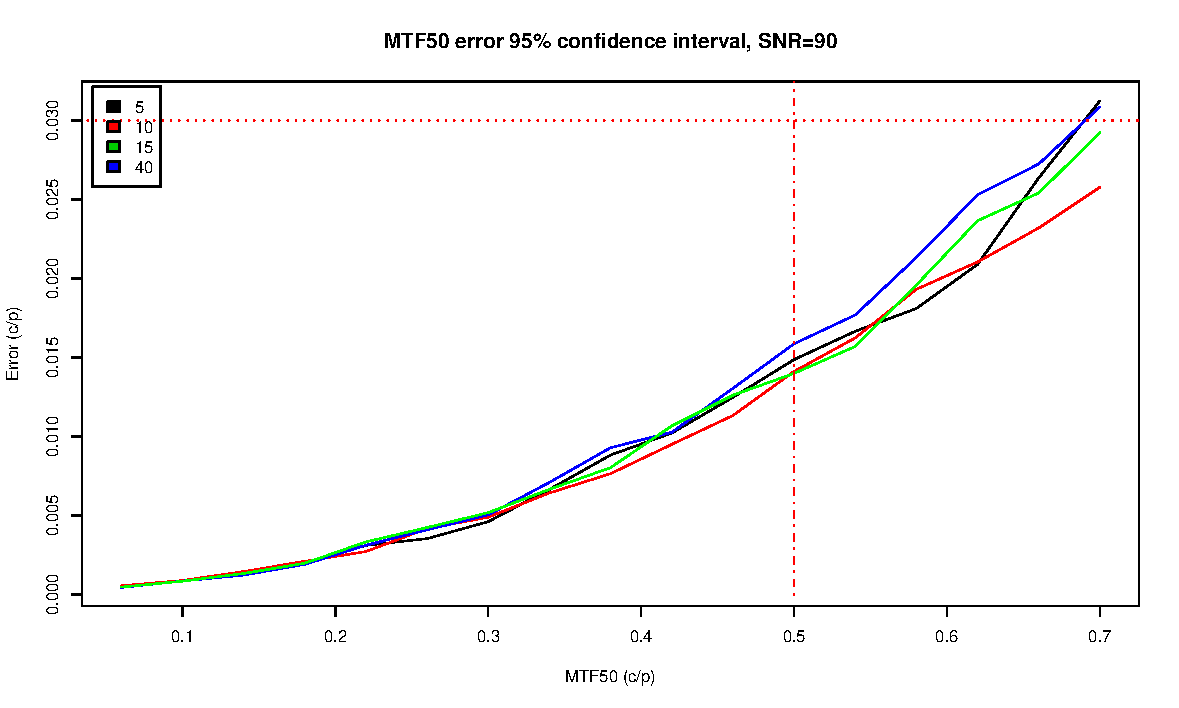
\includegraphics[width=0.95\textwidth]{figures/accuracy_plot_90}
\caption{95\% confidence interval for MTF50 estimate at SNR=90}
\label{fig:mtf_accuracy_snr90}
\end{figure}

\begin{figure}
\centering
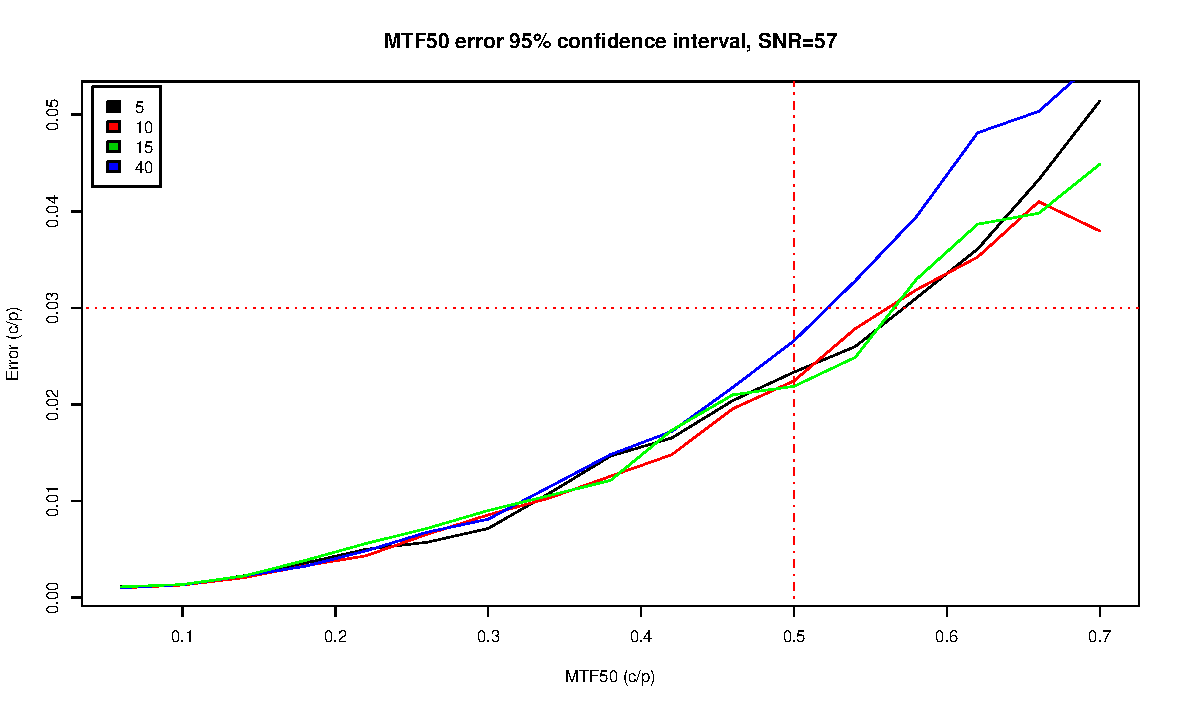
\includegraphics[width=0.95\textwidth]{figures/accuracy_plot_57}
\caption{95\% confidence interval for MTF50 estimate at SNR=57}
\label{fig:mtf_accuracy_snr57}
\end{figure}


Figures~\ref{fig:mtf_accuracy_a10_snr90}--\ref{fig:mtf_accuracy_a10_snr57} present an indication of the error in MTF50
estimates. The following parameters applied:
\begin{enumerate}
  \item Edge length was fixed at 75 pixels.
  \item Two noise levels were investigated: edge contrast at 0.9 times
dynamic range, with noise standard deviation at 0.01 times dynamic range, for an SNR of 90, and
edge contrast at 0.67 with noise at 0.012, for an SNR of 57. The latter case
approximates closely the real world conditions observed with a DSLR camera.
  \item Edge MTF50 values over the range [0.06,0.7) were sampled.
  \item Edge orientations of $2^\circ$ to $44^\circ$ were
explored.
  \item A total 200 data points were collected for each MTF50/angle
combination.
\end{enumerate}
Figures~\ref{fig:mtf_accuracy_a10_snr90}--\ref{fig:mtf_accuracy_a10_snr57}
clearly illustrate how the error increases
with higher edge acuity, especially at slant angles that are further from
ideal. The boxplots are intepreted as follows: the ``whiskers'' indicate the
extreme values observed, although outliers may be excluded and shown
separately as circles; the solid black line in the centre of each box is the
median of the 200 data points, with the red box bounding the 50\%
middle-most values. If this data is expressed as a relative value, i.e., MTF50 error over MTF50
value, then the standard deviation of the relative error is roughly below
1\%, with the extremes hovering around 5\%, up to the Nyquist limit at 0.5
c/p, for the SNR=57 case. The 95\% confidence interval width on the absolute errors are given in
Figures~\ref{fig:mtf_accuracy_snr90} and \ref{fig:mtf_accuracy_snr57}.

Sharp lenses should produce values in the range of (0.2,0.35) cycles per
pixel using unsharpened raw images.  Overall, both absolute accuracy (bias)
and uncertainty (variance) remain fairly well controlled up to the Nyquist
frequency of 0.5 cycles per pixel, but some effort should be expended to
keep the SNR high (i.e., limit image noise) if high accuracy is desired.

\textbf{Warning:} The slanted edge method does not work at all if the edge
acuity is very high (MTF50 of 0.5 and higher) if your edges
are perfectly aligned with the rows or columns of the image. That is why it
is called the \emph{slanted edge} method \ldots. Anyway, MTF mapper does not
currently protect you from this case, and will happily try to measure the
MTF50 across any edge you throw at it. If the MTF50 value exceeds 1.0 c/p,
the program will silently ignore that edge, but poorly oriented edges may
produce very high MTF50 values that are still below 1.0, i.e., a sharp edge at an
angle of $0.5^\circ$ may very well produce an MTF50 value of 0.86. It is
recommended that you ensure that your edges are between $5^\circ$ and
$15^\circ$ degrees with respect to the horizontal or vertical directions.
Some intermediate angles may produce very inaccurate results, e.g.,
$22.5^\circ$ and $45^\circ$ angles are to be avoided at all costs. Future
versions of MTF Mapper may include options to filter out these cases
automatically, but currently you are responsible for keeping edge orientations
reasonable.


\begin{thebibliography}{9}
\bibitem{khom} Kohm, K., \newblock{Modulation transfer function measurement
method and results for the Orbview-3 high resolution imaging
satellite}, \newblock{Congress International Society for Photogrammetry and Remote
Sensing}, 20:12--23, 2004.
\bibitem{bradley} Bradley, D. and Roth, G.,
\newblock{Adaptive thresholding using the integral image},
\newblock{\textit{Journal of Graphics, GPU, \& Game Tools}}, \textbf{12(2)}:13--21,
2007.
\bibitem{chang} Chang, F., Chen, C.J., Lu, C.J.,
\newblock{A linear-time component-labeling algorithm using contour tracing
technique},
\newblock{\textit{Computer Vision and Image Understanding}}, \textbf{93(2)}:206--220,
2004
\end{thebibliography}

\end{document}
